La struttura utilizzata in questo template non è obbligatoria, però ritengo che sia molto comoda per evitare di scrivere file troppo lunghi e di avere un controllo migliore sulla struttura. Questa prevede di scrivere l'introduzione al capitolo in un file salvato nella cartella principale e di sviluppare le sezioni all'interno di una cartella. Esempio di richiamo ad un riferimento \cite{CNN}.

\begin{displayquote}
«\textit{Each thing says what it is...a fruit says ‘Eat me’; water says ‘Drink me’; thunder says ‘Fear me’...}» (Koffka, 1935)
\end{displayquote}

\section{Sezione 1}
Ad ogni sezione, in questo template, corrisponde un file all'interno della cartella relativa al capitolo.

\section{Sezione 2}
Una sezione può contenere una sottosezione. In questo caso, è stato deciso di non creare altri file...

\subsection{Sottosezione}
...ma di scrivere il testo all'interno del file della sezione corrente.

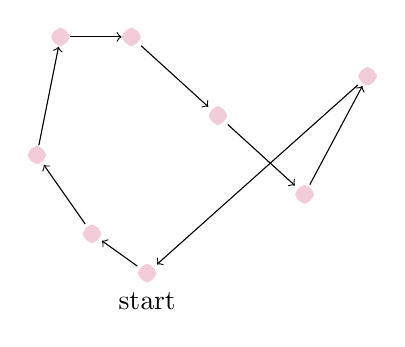
\begin{tikzpicture}
    \tikzstyle{city} = [fill=purple!20,rounded corners]

    \node[city] (A) at (1.3,4.0){};
    \node[city] (B) at (1.6,5.5){};
    \node[city,label=below:start] (C) at (2.7,2.5){};
    \node[city] (D) at (4.7,3.5){};
    \node[city] (E) at (2.0,3.0){};
    \node[city] (F) at (2.5,5.5){};
    \node[city] (G) at (3.6,4.5){};
    \node[city] (H) at (5.5,5){};

    %\draw[->] (C.west) -- (E.east);
    %\draw[->] (B.south) -- (A.east);
    \draw[->] (C) edge (E) (E) edge (A) (A) edge (B) (B) edge (F) (F) edge (G) (G) edge (D) (D) edge (H) (H) edge (C);

\end{tikzpicture}

\begin{algorithm}
    \caption{Farthest Insertion}\label{algo:extramileage}
    \begin{algorithmic}[1]
    \Require $G = (V,E), c:E \to \mathbb{R}^+$
    \Ensure $\text{sub optimal TSP solution}$

    \State $solution \gets$ empty
    \State $cost \gets 0$
    \State $visited \gets  *$ find diameter nodes i-j of G $*$
    \State add ($i$,$j$) and ($j$,$i$) edges to $solution$
    \State $cost \gets cost + 2 c_{ij}$
    


    \While{$\left | visited \right | \neq \left | V  \right |$}
    \State $candidate \gets $ generic node h $ \notin visited$
    \State $candidate \gets *$ find edge i-j visited that minimizes $\Delta = c_{ih} + c_{hj} - c_{ij}*$
    \State $cost \gets cost + \Delta$
    \State remove ($i$,$j$) edge to $solution$
    \State add ($i$,$h$) and ($h$,$j$) edges to $solution$
    \State add $candidate$ to $visited$

    \EndWhile



    \end{algorithmic}
\end{algorithm}

\begin{tikzpicture}
    \tikzstyle{city} = [fill=purple!20,rounded corners]

    \node[city] (A) at (1,5){};
    \node[city] (B) at (2,4){};
    \node[city,label=above:h] (C) at (3,7){};
    \node[city,label=below:j] (D) at (4,1){};
    \node[city,label=above:i] (E) at (6,8){};
    \node[city] (F) at (7,3){};
    \node[city] (G) at (9,6){};

    

    \draw[->] (D) edge[bend right] node [right] {} (E);
    \draw[->] (E) edge[bend right] node [right] {} (D);

    \draw[dashed,->] (E) edge (C) (C) edge (D.west);

    

\end{tikzpicture}

\begin{tikzpicture}
    \tikzstyle{city} = [fill=purple!20,rounded corners]

    \node[city,label=above:a] (A) at (1,5){};
    \node[city,label=below:b] (B) at (1,1){};
    \node[city,label=above:b'] (C) at (5,5){};
    \node[city,label=below:a'] (D) at (5,1){};

    \node[city,label=above:a] (E) at (7,5){};
    \node[city,label=below:b] (F) at (7,1){};
    \node[city,label=above:b'] (G) at (11,5){};
    \node[city,label=below:a'] (H) at (11,1){};

    

    \draw[dashed,->] (C) edge[bend right] node [right] {} (A);
    \draw[dashed,->] (D) edge[bend left] node [left] {} (B);

    \draw[dashed,->] (G) edge[bend right] node [right] {} (E);
    \draw[dashed,->,red] (F) edge[bend left] node [left] {} (H);

    \draw[->] (A) -- (D);
    \draw[->] (B) -- (C);

    \draw[->] (E) -- (F);
    \draw[->] (H) -- (G);
    


    %\draw[dashed,->] (E) edge (C) (C) edge (D.west);

    

\end{tikzpicture}
